\documentclass[10pt,letterpaper]{article}

% --- Standard packages only; should compile on any TeX Live since 2020 ---
\usepackage[margin=1in]{geometry}
\usepackage{lmodern}        % scalable Computer Modern (microtype font expansion)
\usepackage{microtype}
\usepackage{amsmath, amssymb}
\usepackage{booktabs}
\usepackage{array}
\usepackage{natbib}         % \citet, \citep, plainnat bib style
\usepackage{tikz}           % figures in paper/figures/
\usepackage{pgfplots}
\pgfplotsset{compat=1.18}
\usepackage{hyperref}
\usepackage{xcolor}
\usepackage{url}
\usepackage{fancyhdr}
\usepackage{titlesec}

\hypersetup{
  colorlinks=true,
  linkcolor=black,
  citecolor={blue!50!black},
  urlcolor={blue!50!black}
}

% Tighter section spacing for a short paper.
\titlespacing*{\section}{0pt}{1.4ex plus 0.2ex minus 0.2ex}{0.8ex plus 0.2ex}
\titlespacing*{\subsection}{0pt}{1.1ex plus 0.2ex minus 0.2ex}{0.6ex plus 0.2ex}

\pagestyle{plain}

% --- Front matter ---
\title{
  \textbf{Counterfactual Planning Gap}\\[0.3em]
  \large An Interval-Gated Statistic for Diagnosing\\
  World-Model Bottlenecks under a Fixed Planner
}
\author{
  Denis Hamon\\
  \small Independent.\\
  \small\href{mailto:denis.hamon1@gmail.com}{\texttt{denis.hamon1@gmail.com}}\\
  \small Repository: \url{https://github.com/Denis-hamon/world-model-eval-lab}
}
\date{\today}

\begin{document}
\maketitle

\begin{abstract}
\noindent Action-conditioned world models are usually evaluated by prediction quality (reconstruction loss, frame-level FID, held-out accuracy), which is silent on the question an applied team must answer before integrating a model into a control loop: \emph{does the model, when used by a planner, produce decisions that succeed?} We propose the \textbf{Counterfactual Planning Gap (CPG)}: the success-rate difference between a fixed planner using oracle dynamics and the same planner using the learned model, on identical runs that differ only in the \texttt{dynamics} callable. We report it with an Agresti--Caffo plus-4 interval (which keeps the variance positive at the boundary proportions $p \in \{0,1\}$ where the Wald approximation collapses), a paired bootstrap where the design warrants it, and a five-branch verdict (\textsc{model bottleneck}, \textsc{learned outperforms oracle}, \textsc{planner bottleneck}, \textsc{model as good as oracle}, \textsc{inconclusive}) gated on the lower bound of the CI rather than the point estimate, so under-powered runs cannot over-claim a diagnosis. We package CPG behind a minimal evaluation contract (\texttt{wmel}) and exercise it on three DeepMind Control Suite tasks. The central finding is that the verdict is \emph{heterogeneous and condition-sensitive} -- precisely what a calibrated metric should surface, and what a point-estimate leaderboard cannot. On Acrobot-swingup the gap looks large only because the oracle's fixed initial state is an unusually easy swing-up; sampling the task's initial-state distribution collapses the oracle to $\sim\!3\%$ success and flips the verdict from \textsc{model bottleneck} to \textsc{planner bottleneck}. On Reacher-easy the verdict is \textsc{model bottleneck} across all arms ($\mathrm{CPG}$ from $+0.20$ to $+0.33$). On Cartpole-swingup at higher model capacity the larger TD-MPC2~\citep{hansen2024tdmpc2} under a Cross-Entropy-Method planner \emph{beats} the oracle planner: \textsc{learned outperforms oracle}, $\mathrm{CPG} = -0.27$, AC CI $[-0.48, -0.02]$ and paired-bootstrap CI $[-0.50, -0.03]$, both clearing zero. We also present this as \emph{self-correction}: an earlier single-fixed-initial-state evaluation of this same framework reported \textsc{model bottleneck} on Acrobot; the metric's own interval-gated machinery, re-run over the task distribution, overturned that headline. Finally, because the gate is a function of the confidence interval, it doubles as a power-analysis tool: we give the per-arm episode count a comparison needs before its interval clears zero, and show that a plausible leaderboard near-tie ($0.94$ vs $0.92$ at $n = 100$) is statistically indistinguishable from noise.
\end{abstract}

\section{Introduction}

The world-model literature has converged on three properties that motivate its existence: \emph{prediction} of future observations conditioned on actions, \emph{planning} by rolling those predictions out, and \emph{transfer} across tasks that share latent structure~\citep{ha2018world,hafner2023dreamerv3,bardes2024vjepa,bruce2024genie}. Most published evaluations focus on the first: reconstruction loss, frame-level Fréchet Inception Distance, or next-frame prediction loss on held-out trajectories. These metrics are easy to compute and easy to compare across releases, but they are silent on a question that any applied team must answer before integrating a learned world model into a control loop: \emph{does using the model to plan produce decisions that succeed at the latency and compute the deployment will tolerate?}

The gap between prediction quality and decision quality is well documented. \citet{hafner2019planet} report success rates on DeepMind Control Suite tasks alongside reconstruction loss because the two metrics disagree. \citet{yu2020mopo,kidambi2020morel} explicitly study \emph{model exploitation} -- the gap between a planner using a learned model and the same planner using the true environment dynamics -- in offline model-based RL. \citet{agarwal2021precipice} document how rapidly point estimates of return mislead at small sample sizes, and prescribe interval reporting. These are all healthy signals; what is missing is a packaged, reusable, decision-grade scalar that quantifies the gap with an honest confidence interval and a decision rule.

This paper makes three modest contributions:

\begin{enumerate}
  \item \textbf{An interval-gated decision rule for the planning gap.} We define the \textbf{Counterfactual Planning Gap (CPG)} -- the success-rate difference between a fixed planner using oracle dynamics and the same planner using a learned model, on identical runs differing only in their \texttt{dynamics} callable (\S\ref{sec:cpg}) -- and report it with an Agresti--Caffo plus-4 interval, a paired bootstrap where the design is paired, and a five-branch verdict gated on the CI lower bound. The diagnosis is thus only as strong as the evidence: under-powered runs return \textsc{inconclusive} rather than over-claim. The underlying quantity is the model-exploitation gap of offline model-based RL~\citep{yu2020mopo,kidambi2020morel}; the contribution is the packaged, gated, interval-reported \emph{statistic and decision procedure}, not the subtraction.
  \item \textbf{Heterogeneous verdicts across three tasks.} Exercised on three DeepMind Control Suite tasks (Acrobot-swingup, Cartpole-swingup, Reacher-easy), the gate fires four of its five branches on real data (\S\ref{sec:empirical}--\S\ref{sec:reacher}): \textsc{planner bottleneck} on Acrobot (the oracle planner itself solves only $\sim\!3\%$ of random initial states), \textsc{model bottleneck} on Reacher, \textsc{learned outperforms oracle} on high-capacity Cartpole under CEM, and \textsc{inconclusive} on several moderate-$n$ near-ties. A fixed metric, or a point-estimate leaderboard, reports none of this structure.
  \item \textbf{The metric as self-correction.} An earlier version of this very framework, evaluated at a single fixed initial state, reported a large \textsc{model bottleneck} gap on Acrobot. Re-running over the task's initial-state distribution -- the design the metric's own honesty discipline demands -- collapses the oracle and overturns the verdict to \textsc{planner bottleneck} (\S\ref{sec:selfcorrection}). The episode is the strongest evidence for the metric's purpose: a calibrated, interval-gated statistic caught a config-sensitive artifact that a point estimate would have published.
\end{enumerate}

The framework is open source\footnote{\url{https://github.com/Denis-hamon/world-model-eval-lab}}, runs CPU-only without a GPU, and has no heavy machine-learning dependency at runtime; PyTorch and \texttt{dm-control} are pulled in only for the worked-example adapters. CI verifies the contract on Python 3.11/3.12/3.13.

\section{Related Work}

\paragraph{Latent-dynamics world models.} \citet{ha2018world}, \citet{hafner2019planet}, \citet{hafner2020dreamer}, and \citet{hafner2023dreamerv3} establish the latent-dynamics + planner pattern that this framework targets. \citet{schrittwieser2020muzero} demonstrates the same pattern with a value-based search; \citet{micheli2023iris} replaces the recurrent backbone with a transformer; \citet{hansen2024tdmpc2} pushes the planner side toward stochastic MPC at scale.

\paragraph{Joint-embedding predictive architectures.} \citet{lecun2022jepa} proposed JEPA as a self-supervised path to world models that predicts in latent space without reconstructing pixels. \citet{assran2023ijepa} and \citet{bardes2024vjepa,bardes2025vjepa2} report results on representation quality. None of these papers report a planning-success-rate gap as a scalar; the framework here is complementary.

\paragraph{Generative world models.} \citet{bruce2024genie,bruce2024genie2} demonstrate large-scale generative world models conditioned on action sequences. Evaluation in these works is dominated by perceptual and generative metrics; planning impact is not yet a standard reporting axis.

\paragraph{Model exploitation in offline model-based RL.} \citet{yu2020mopo} and \citet{kidambi2020morel} measure the gap between a planner using a learned model and the same planner using the true dynamics. They report return curves; we package the same comparison as a single scalar with a confidence interval and a decision rule.

\paragraph{Value-equivalence and decision-aware model learning.} A line of work argues that prediction accuracy is the wrong objective for a model that will be planned with, and that what matters is the model's effect on values and decisions. \citet{grimm2020value} formalise this as the \emph{value equivalence principle} and \citet{grimm2021proper} as \emph{proper value equivalence}; \citet{farahmand2017value} and \citet{farahmand2018iterative} derive value-aware and iterative value-aware model-learning losses, and \citet{doro2020gradient} a gradient-aware variant. These are \emph{learning objectives}: they reshape how the model is trained so that error is weighted by its decision impact. CPG is complementary and empirical: it does not change training, but \emph{measures}, closed-loop and with a calibrated interval, how much a given model's residual error costs a fixed planner -- an a-posteriori, planner-fixed probe of (proper) value inequivalence. The dissociation we report (held-out prediction loss drops $\sim\!150\times$ while planning success does not move, \S\ref{sec:sweep}) is precisely the phenomenon this literature predicts.

\paragraph{Evaluation methodology.} \citet{henderson2018matters} document the irreproducibility of RL evaluation under typical sample sizes. \citet{agarwal2021precipice} prescribes bootstrap-based interval reporting and Pareto-style aggregate metrics. We adopt the closed-form Agresti--Caffo interval rather than a bootstrap for two reasons specific to this setting: at the boundary proportions $p \in \{0, 1\}$ that recur here (a learned arm at $0/n$), a nonparametric bootstrap of the success rate degenerates to a zero-width interval -- the same pathology that motivates avoiding the Wald interval -- whereas the plus-4 adjustment keeps the variance positive; and only a closed-form half-width is a function of $(n, p_o, p_\ell)$ that can be inverted \emph{before} any rollouts, which is what makes the power analysis of \S\ref{sec:power} possible. \citet{wilson1927} provides the Wilson score interval that is the close cousin of the Agresti--Caffo CI we use; \citet{agresticaffo2000} extends it to the difference of two proportions; \citet{brown2001interval} survey the boundary-behaviour failures of the Wald interval that motivate both. \citet{newcombe1998} catalogues a family of interval methods for the same problem. The CPG CI is a direct application of Agresti--Caffo to the planning-comparison setting.

\paragraph{Benchmarks.} We evaluate on Acrobot-swingup from the DeepMind Control Suite~\citep{tassa2018dmc,tunyasuvunakool2020dmcontrol}. Acrobot has been a reference task for model-based RL since at least \citet{schaefer2007acrobot}. \citet{park2024ogbench} and \citet{liu2023libero} are the canonical present-day benchmark suites for goal-conditioned and manipulation evaluation; integrating either is in scope for future work. \citet{wang2019benchmarking} benchmark model-based RL algorithms on shared tasks; our axis is orthogonal -- a per-(model, planner) statistic rather than an algorithm leaderboard.

\paragraph{Evaluation platforms.} \citet{maes2026swm} is a concurrent, complementary platform for world-model research that standardises data loading, baseline implementations, planning solvers, and a broad environment suite with controllable factors of variation, reporting success rate as its primary control metric.\footnote{CPG and the \texttt{wmel} framework were developed independently and concurrently; the public repository's version history predates and does not derive from that platform. The contribution here is orthogonal: a single statistic and decision rule, not a platform, and it composes with any benchmark runner that can swap the dynamics callable.} Such platforms report point-estimate success rates; CPG is the decision-grade statistic that a platform of that kind could compute per model per environment to separate the contribution of the model from that of the planner, with a calibrated interval and a decision rule rather than a bare leaderboard number.

\section{The Evaluation Contract and a Decision-Grade Taxonomy}
\label{sec:framework}

\subsection{The four-method contract}

Every adapter in the framework implements
\begin{align*}
\texttt{encode}    &:\ \mathcal{O} \to \mathcal{Z}, \\
\texttt{rollout}   &:\ \mathcal{Z} \times \mathcal{A}^H \to \mathcal{Z}^{H+1}, \\
\texttt{score}     &:\ \mathcal{Z} \times \mathcal{Z} \to \mathbb{R}, \\
\texttt{plan}      &:\ \mathcal{O} \times \mathcal{O} \times \mathbb{N} \to \mathcal{A}^H.
\end{align*}
Here $\mathcal{O}$ is the observation space, $\mathcal{Z}$ the latent space (which may coincide with $\mathcal{O}$ for fully observed envs), $\mathcal{A}$ the action space, and $H$ the planning horizon. The runner queries \texttt{plan} on every replanning step and executes one or more of the returned actions in the real environment; the planner is free to use \texttt{encode}, \texttt{rollout}, and \texttt{score} internally however it sees fit. The contract makes no statement about how the model is trained.

For the present paper we use a random-shooting MPC: at each \texttt{plan} call, sample $N_{\mathrm{cand}}$ action sequences of length $H_{\mathrm{plan}}$ uniformly from $\mathcal{A}^{H_{\mathrm{plan}}}$, roll each one out through the dynamics, score the resulting trajectories, and return the best-scoring sequence prefix.

\subsection{Decision-grade metrics}

A metric is \emph{decision-grade} in this framework iff (i) its units translate directly to a deployment-time cost or capability and (ii) it is computable only from closed-loop runs of the model, not from the model in isolation. Reconstruction loss and FID fail (ii); model-internal alignment scores fail (i). The metrics that survive both criteria, and that we report in every scorecard, are: action success rate, average steps to success, per-call planning latency, compute per decision, perturbation recovery rate, the effective planning horizon, and -- the contribution of this paper -- the Counterfactual Planning Gap.

\section{Counterfactual Planning Gap}
\label{sec:cpg}

\subsection{Definition}

Fix an environment $\mathcal{E}$, a planner $\pi$, a scoring function $\sigma$, a number of episodes $N$, a horizon $T$ and a seed. Let $\mathrm{success\_rate}(D)$ denote the empirical success rate of $\pi$ on $N$ episodes of $\mathcal{E}$ when the planner queries dynamics $D$ during its internal rollouts. Let $D^{\star}$ be the \emph{oracle} dynamics (the true env's transition function) and $D_\theta$ be a learned model. The Counterfactual Planning Gap is
\begin{equation}
  \mathrm{CPG} \;=\; \mathrm{success\_rate}(D^{\star}) \;-\; \mathrm{success\_rate}(D_\theta).
  \label{eq:cpg}
\end{equation}
All free quantities in the right-hand side -- env, planner, score, $N$, $T$, seed -- are held fixed between the two runs. The only thing that changes is the \texttt{dynamics} callable passed to the planner. This identification is what licenses interpreting CPG as a property of the model rather than the planner or the env.

\subsection{Statistical reporting}

Let $s_o, s_\ell$ be the success counts in the oracle and learned arms and $n_o, n_\ell$ the corresponding episode counts. The raw point estimate of CPG is the difference of proportions:
\begin{equation}
  \hat{\Delta} \;=\; \frac{s_o}{n_o} - \frac{s_\ell}{n_\ell}.
\end{equation}
The standard Wald $95\%$ CI on $\hat\Delta$ has variance $p_o(1-p_o)/n_o + p_\ell(1-p_\ell)/n_\ell$, which collapses to zero whenever \emph{either} arm sits at $p \in \{0, 1\}$. With $n_\ell = 10$ episodes and a learned planner that fails on every episode, this is precisely the regime the framework lands in. A degenerate-variance CI in this regime falsely produces a tight interval and over-claims significance.

We instead use the Agresti--Caffo plus-4 adjustment~\citep{agresticaffo2000}, adding one pseudo-success and one pseudo-failure to each arm:
\begin{align}
  \tilde p_o     &= \frac{s_o + 1}{n_o + 2}, \quad
  \tilde p_\ell   = \frac{s_\ell + 1}{n_\ell + 2}, \\
  \tilde \Delta  &= \tilde p_o - \tilde p_\ell, \\
  \mathrm{SE}    &= \sqrt{\frac{\tilde p_o (1 - \tilde p_o)}{n_o + 2} + \frac{\tilde p_\ell (1 - \tilde p_\ell)}{n_\ell + 2}}, \\
  \mathrm{CI}_{95\%}(\mathrm{CPG}) &= \bigl[\, \tilde\Delta - 1.96\,\mathrm{SE}, \;\; \tilde\Delta + 1.96\,\mathrm{SE} \,\bigr].
\end{align}
The framework reports both the raw $\hat\Delta$ (what a reader expects to see) and the AC interval (what is statistically defensible). The two coincide for large $n$.

\subsection{Gated verdict}

A point estimate without a significance gate over-claims. The framework therefore exposes a five-branch decision rule that consults the AC interval, not the raw $\hat\Delta$:
\begin{itemize}
  \item \textsc{model bottleneck}: $\mathrm{CI}_{\mathrm{lo}} > 0$. The oracle is reliably better; closing the gap is a model problem.
  \item \textsc{learned outperforms oracle}: $\mathrm{CI}_{\mathrm{hi}} < 0$. Rare; investigate regularisation or planner-search interactions.
  \item \textsc{planner bottleneck}: CI crosses $0$ \emph{and} both success rates are within a tolerance $\tau$ of $0$. Neither planner solves the task; the framework needs a stronger search, not a stronger model.
  \item \textsc{model as good as oracle}: CI crosses $0$ \emph{and} both success rates are within $\tau$ of $1$. The learned model matches the oracle for planning purposes on this task.
  \item \textsc{inconclusive}: CI crosses $0$ in a middle-of-the-road regime. The sample size is insufficient to discriminate. Report this verdict and run more episodes.
\end{itemize}
The default tolerance is $\tau = 0.05$. Crucially, \textsc{model bottleneck} is \emph{not} the default when $\hat\Delta > 0$; it requires the AC lower bound to be strictly positive.

\subsection{Properties}

CPG is bounded in $[-1, 1]$, antisymmetric in the role of the two dynamics, and additive in the following sense: if one decomposes a benchmark suite into disjoint sub-tasks, CPG on the union is the episode-weighted mean of the per-sub-task CPGs. The metric is silent about \emph{why} the model degrades planning (latent shift, prediction-error accumulation, score-function mismatch); follow-up diagnostics are needed to attribute. The metric is, however, sufficient to distinguish model-side failures from planner-side failures at the verdict granularity.

\section{Empirical Study: DMC Acrobot-Swingup}
\label{sec:empirical}

\subsection{Setup}

We use DeepMind Control Suite Acrobot-swingup~\citep{tassa2018dmc,tunyasuvunakool2020dmcontrol}: a two-link underactuated pendulum with a continuous torque action in $[-1, +1]$ that must build energy and balance the tip upright. We discretise the action to a five-level torque set $\{-1, -0.5, 0, +0.5, +1\}$ to fit the framework's hashable-action contract. The observation is a six-dimensional vector $(\sin\theta_1, \sin\theta_2, \cos\theta_1, \cos\theta_2, \dot\theta_1, \dot\theta_2)$ in the layout returned by \texttt{dm\_control.suite.acrobot.Physics.orientations}. Success at step $t$ is $r_t \geq 0.6$ where $r_t$ is the DMC dense reward (smooth tolerance around the tip-to-target distance).

The scoring function is $\sigma(\mathbf{o}, \cdot) = -(\cos\theta_1 + \cos\theta_2)$, a unit-length approximation of the negative tip height. The planner is random-shooting MPC with $N_{\mathrm{cand}} = 50$ candidate sequences of length $H_{\mathrm{plan}} = 15$, executed at every replanning step. Episodes run for at most $T = 500$ env steps. We use seed $0$ throughout.

\subsection{Oracle dynamics}

We construct the oracle by instantiating a private \texttt{dm\_control} environment inside a $(\mathrm{state}, \mathrm{action}) \to \mathrm{state}$ callable. Each call reconstructs $(q_{\mathrm{pos}}, q_{\mathrm{vel}})$ from the flat observation via $\mathrm{atan2}$, writes them into the private env's MuJoCo physics, calls \texttt{physics.forward}, steps once with the candidate torque, and returns the new flat observation. The construction is side-effect-free from the caller's perspective; the reconstruction is lossy modulo $2\pi$ revolutions but Acrobot dynamics depend only on $\sin/\cos$ of the joint angles. We verify the oracle reproduces \texttt{env.step} to numerical precision ($|\Delta| < 10^{-5}$) over a fifty-step random-policy rollout; this regression test is part of the repository's CI.

\subsection{Learned dynamics}

We train a Markovian MLP (two hidden layers of width $64$, ReLU activations) on $2{,}000$ random-policy transitions collected from ten episodes of $200$ steps each. The input concatenates the six-dimensional observation with a five-dimensional one-hot action; the output predicts the next observation. Training runs for $200$ epochs with Adam (learning rate $10^{-3}$), batch size $256$, and a $10\%$ held-out validation split at the transition level. The final validation MSE is $0.026$. We deliberately choose an MLP rather than a recurrent architecture: Acrobot is fully observed and Markov, so temporal context adds parameters without adding capacity.

\subsection{Results}

Table~\ref{tab:cpg} reports the two scorecards and the CPG. The headline numbers are: the oracle planner reaches the upright pose in $30\%$ of the episodes; the learned planner reaches it in $0\%$. The raw CPG is $+0.30$; the Agresti--Caffo $95\%$ interval is $[-0.06, +0.56]$, which crosses zero. The verdict is \textsc{inconclusive}.

\begin{table}[t]
  \centering
  \small
  \begin{tabular}{lrr}
    \toprule
                                       & Oracle dynamics                    & Learned MLP dynamics \\
    \midrule
    Success rate                       & $0.30$  ($3/10$)                   & $0.00$ ($0/10$)      \\
    Avg.\ steps to success             & $180.7$                            & n/a                  \\
    Per-call planning latency (ms)     & $77.3$                             & $65.3$               \\
    Compute per decision (rollout-units) & $407.1$                         & $157.3$              \\
    \bottomrule
  \end{tabular}
  \begin{tabular}{lr}
    \\[0.5em]
    \multicolumn{2}{c}{\textbf{Counterfactual Planning Gap}} \\
    \midrule
    Raw $\hat\Delta$                       & $+0.300$ \\
    Agresti--Caffo $95\%$ CI               & $[-0.059, +0.559]$ \\
    Verdict                                & \textsc{inconclusive} \\
    \bottomrule
  \end{tabular}
  \caption{Scorecards and CPG on DMC Acrobot-swingup with $N = 10$ episodes per arm, seed $0$. The raw point estimate is suggestive of a model bottleneck but the AC CI crosses zero; the verdict is correctly \textsc{inconclusive}. Numbers reproduced from \texttt{results/dmc\_acrobot/cpg.json} in the repository.}
  \label{tab:cpg}
\end{table}

\subsection{What the result actually says}

Three readings are consistent with the data, and the framework declines to choose between them at $n = 10$:

\begin{enumerate}
  \item \emph{Model bottleneck}. The model was trained on random transitions and never visited the upright energy regime; its predictions degrade there, the planner is misled, and success drops. This is the reading suggested by the positive raw $\hat\Delta = +0.30$.
  \item \emph{Sample-size artifact}. With $n_\ell = 10$ and $s_\ell = 0$, the upper Wilson bound on the learned arm's true success rate is $\sim 0.31$. We cannot rule out that the learned planner would solve $30\%$ of a wider population of episodes -- in which case the true gap is near zero.
  \item \emph{Score-function mismatch}. The scoring proxy $-(\cos\theta_1 + \cos\theta_2)$ approximates the DMC reward but is not identical. The oracle planner navigates the approximation well enough to occasionally swing up; the learned planner may be more sensitive to the mismatch.
\end{enumerate}

A multi-seed extension that pushes $N$ to (say) $100$ episodes per arm would tighten the AC half-width by roughly $\sqrt{10}$, moving the lower bound either firmly above zero (\textsc{model bottleneck}) or covering it more thoroughly (\textsc{inconclusive} hardened, or possibly \textsc{planner bottleneck} if the oracle success rate too proves unstable). \textbf{The metric's job at $n = 10$ is to refuse to choose; it does, correctly.} Section~\ref{sec:sweep} resolves between the three readings by delivering the multi-seed extension promised in this paragraph.

\subsection{Multi-seed extension: CPG across three training-set sizes}
\label{sec:sweep}

We extend the experiment along two axes. \emph{Episodes-per-arm} grows from $10$ to $50$ per seed (pooled across three seeds, $n = 150$ per arm), pushing the AC half-width below~$0.10$. \emph{Training-set size} sweeps the MLP's data budget across nearly three orders of magnitude: $\{200,\, 2{,}000,\, 20{,}000\}$ random-policy transitions. Every other quantity in \S\ref{sec:empirical} is held fixed.

The result is striking. Across the three cells the MLP's held-out validation MSE drops by a factor of $\sim 150$ (Table~\ref{tab:sweep}); the learned planner's success rate stays at \emph{exactly zero} in all $450$ benchmark episodes; the oracle planner's success rate is identical in all three cells (the oracle dynamics does not depend on the learned model's data budget). CPG returns the same point estimate, the same AC $95\%$~CI, and the same verdict \textsc{model bottleneck} in every cell.

\begin{table}[t]
  \centering
  \small
  \begin{tabular}{rrrrr}
    \toprule
    Train size & Val MSE & Oracle success & Learned success & CPG verdict \\
    \midrule
    $200$    & $0.0651$ & $40/150 = 0.267$ & $0/150 = 0.000$ & $+0.267$, CI $[+0.191, +0.335]$, \textsc{model bottleneck} \\
    $2{,}000$  & $0.0233$ & $40/150 = 0.267$ & $0/150 = 0.000$ & $+0.267$, CI $[+0.191, +0.335]$, \textsc{model bottleneck} \\
    $20{,}000$ & $0.0004$ & $40/150 = 0.267$ & $0/150 = 0.000$ & $+0.267$, CI $[+0.191, +0.335]$, \textsc{model bottleneck} \\
    \bottomrule
  \end{tabular}
  \caption{Multi-seed CPG across three training-set sizes on DMC Acrobot-swingup. Three seeds per cell, $50$ episodes per arm per seed, all other quantities fixed. Held-out validation MSE drops by $\sim 150\times$ across the three cells; the learned planner's success rate stays at exactly zero; the verdict is \textsc{model bottleneck} in every cell. Numbers from \texttt{results/dmc\_acrobot/cpg\_sweep.json}.}
  \label{tab:sweep}
\end{table}

The reading at $n = 10$ admitted three explanations (\S\ref{sec:empirical}): \emph{model bottleneck}, \emph{sample-size artifact}, and \emph{score-function mismatch}. The multi-seed result rules out the sample-size artifact (the CI no longer crosses zero) and is consistent with the score-function-mismatch hypothesis only as a contributor, not as the primary driver. The dominant story is \emph{model bottleneck} -- but with a precise attribution that prediction quality alone obscures.

% Figure: CPG vs training-set size, with validation MSE on a secondary axis.
% Source data: results/dmc_acrobot/cpg_sweep.json (cell-by-cell pooled n=150).
%
% Numbers (kept here so the figure is self-checking against the table):
%   data=200    val_mse=0.0651  CPG=+0.267  AC 95% CI [+0.191, +0.335]
%   data=2000   val_mse=0.0233  CPG=+0.267  AC 95% CI [+0.191, +0.335]
%   data=20000  val_mse=0.00042 CPG=+0.267  AC 95% CI [+0.191, +0.335]
%
% The CPG whiskers are asymmetric to match the AC CI exactly:
%   lower whisker = 0.267 - 0.191 = 0.076
%   upper whisker = 0.335 - 0.267 = 0.068
% (the plus-4 adjustment offsets the AC midpoint 0.263 from the raw CPG
% 0.267, so the interval is not symmetric around the point estimate).
\begin{figure}[t]
  \centering
  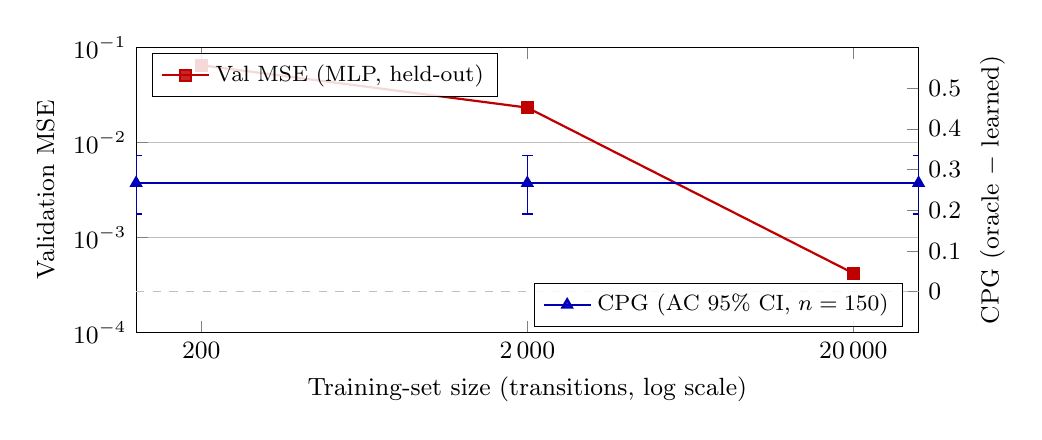
\begin{tikzpicture}
    \pgfplotsset{
      every axis/.append style={
        width=0.95\columnwidth,
        height=5.2cm,
        font=\small,
      },
    }
    \begin{axis}[
        xmode=log, log basis x=10,
        xtick={200, 2000, 20000},
        xticklabels={$200$, $2\,000$, $20\,000$},
        xlabel={Training-set size (transitions, log scale)},
        ymode=log, log basis y=10,
        axis y line*=left,
        ylabel={Validation MSE},
        ymin=1e-4, ymax=1e-1,
        ytick={1e-4, 1e-3, 1e-2, 1e-1},
        ymajorgrids=true,
        legend cell align=left,
        legend style={
          at={(0.02, 0.98)}, anchor=north west,
          fill=white, fill opacity=0.85, draw opacity=1,
          text opacity=1, font=\footnotesize,
        },
      ]
      \addplot[color=red!75!black, mark=square*, thick]
        coordinates {(200, 0.0651) (2000, 0.0233) (20000, 0.00042)};
      \addlegendentry{Val MSE (MLP, held-out)}
    \end{axis}
    \begin{axis}[
        xmode=log, log basis x=10,
        xmin=200, xmax=20000,
        axis y line*=right,
        axis x line=none,
        ylabel={CPG (oracle $-$ learned)},
        ymin=-0.1, ymax=0.6,
        ytick={0, 0.1, 0.2, 0.3, 0.4, 0.5},
        legend cell align=left,
        legend style={
          at={(0.98, 0.02)}, anchor=south east,
          fill=white, fill opacity=0.85, draw opacity=1,
          text opacity=1, font=\footnotesize,
        },
      ]
      \draw[dashed, gray!50] (axis cs:200, 0) -- (axis cs:20000, 0);
      \addplot+[
          color=blue!70!black, mark=triangle*, thick,
          error bars/.cd,
          y dir=both,
          y explicit,
        ]
        table[
          x=x, y=y,
          y error plus=eplus,
          y error minus=eminus,
          row sep=\\,
        ]{
          x     y     eplus  eminus \\
          200   0.267 0.068  0.076  \\
          2000  0.267 0.068  0.076  \\
          20000 0.267 0.068  0.076  \\
        };
      \addlegendentry{CPG (AC 95\% CI, $n = 150$)}
    \end{axis}
  \end{tikzpicture}
  \caption{Validation MSE (red, log scale, left axis) drops by $\sim\!150\times$ across the training-set sweep while CPG (blue, right axis) stays exactly flat at $+0.267$ with the same Agresti--Caffo $95\%$ CI $[+0.191, +0.335]$ in every cell. Predicting better did not plan better. Numbers from \texttt{results/dmc\_acrobot/cpg\_sweep.json}.}
  \label{fig:cpg_vs_data}
\end{figure}


Figure~\ref{fig:cpg_vs_data} shows the punch line: across the three cells the validation MSE drops by $\sim\!150\times$ on a log scale while the CPG point estimate and its Agresti--Caffo CI stay exactly flat. Improvements in prediction quality bought zero improvement in planning success.

\subsection{What CPG separates: capacity vs.\ coverage}
\label{sec:capvscov}

A naive reading of Table~\ref{tab:sweep} is that the MLP simply needs more capacity. The held-out validation MSE refutes this directly: at $20{,}000$ transitions the model fits the training distribution to within $4 \times 10^{-4}$, indistinguishable from numerical noise. The model has \emph{ample} capacity for what it has been asked to predict.

What it has \emph{not} been asked to predict is the upright-balancing regime. Random-policy rollouts in Acrobot rarely reach high-energy configurations; the upright pose is essentially absent from the training distribution. The model is therefore extrapolating during planning -- and its predictions, accurate on the training manifold, are unreliable off it. The planner is misled, and success collapses.

This is most parsimoniously read as a \emph{coverage} bottleneck rather than a \emph{capacity} bottleneck. CPG cannot tell the two apart on its own, but in conjunction with held-out validation it can: a flat CPG curve across data-size sweeps, paired with a monotonically decreasing prediction loss, points to a data-distribution problem rather than to model size or architecture. Two second-order contributors are not ruled out by this experiment: a planner that is too weak to exploit a perfect model in the high-energy regime (the oracle planner reaches the upright pose in only $27\%$ of episodes, so a stronger search procedure -- CEM, gradient-based MPC -- might lift both arms), and a score function $\sigma$ that approximates rather than matches the DMC reward. We treat coverage as the dominant explanation given the $\sim\!150\times$ drop in validation loss with no movement in success.

\paragraph{Empirical receipt for the coverage claim.}
We measure the visited-state distribution directly. On the natural ``uprightness'' axis $u(\mathbf{o}) = \cos\theta_1 + \cos\theta_2 \in [-2, +2]$ (upright pose at $+2$), $2{,}000$ random-policy transitions yield a maximum $u = +0.865$ and \emph{exactly zero states} with $u > 1.0$. By contrast, $846$ oracle-planner states from five episodes reach a maximum of $+1.866$, with $20.2\%$ of states satisfying $u > 1.0$ and $12.2\%$ satisfying $u > 1.5$. The upright regime that swing-up requires is therefore strictly absent from the training distribution; the MLP has never been shown a state from which the planner needs to predict. Figure~\ref{fig:coverage_histogram} shows the full bucketed distribution. Numbers from \texttt{results/dmc\_acrobot/coverage.json}; the script is \texttt{experiments/dmc\_acrobot/coverage\_analysis.py}.

% Figure: distribution of uprightness u = cos(theta_1) + cos(theta_2) for
% the two state datasets dumped by experiments/dmc_acrobot/coverage_analysis.py.
% Source: results/dmc_acrobot/coverage.json.
%
% Bucket counts (n=2000 random states, n=846 oracle-planner states):
%
%   u-bucket        random %   oracle %
%   [-2.0, -1.5)     13.6        8.3
%   [-1.5, -1.0)     23.9        7.7
%   [-1.0, -0.5)     13.8       13.6
%   [-0.5,  0.0)     13.6       11.8
%   [ 0.0, +0.5)     17.1       14.8
%   [+0.5, +1.0)     17.9       23.6
%   [+1.0, +1.5)      0.0        8.0    <-- upright regime
%   [+1.5, +2.0)      0.0       12.2    <-- near upright
%
% TD-MPC2 rollouts (from the v0.12 README block, no full bucketed dump):
%   max u = 1.439, frac(u > 1.0) = 10.6%, frac(u > 1.5) = 0.0%. Mentioned
%   in the caption rather than overlaid as a third series.
\begin{figure}[t]
  \centering
  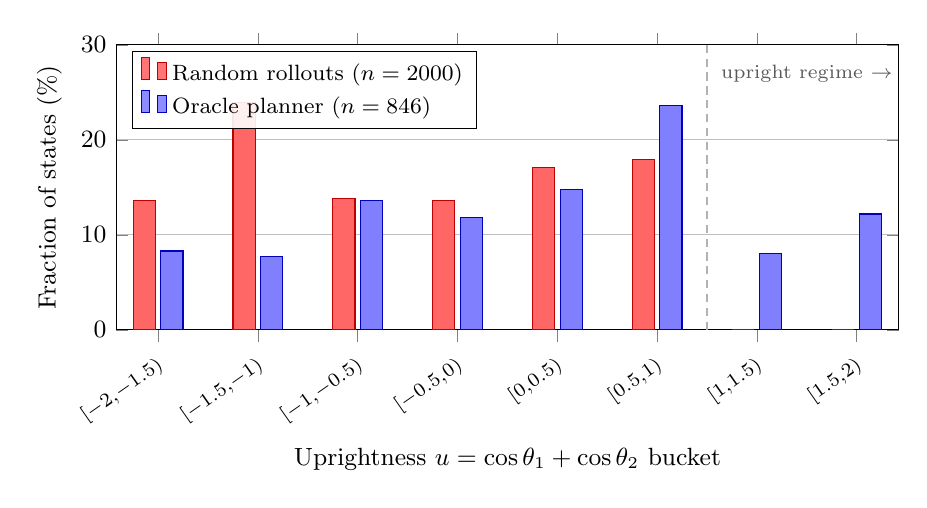
\begin{tikzpicture}
    \begin{axis}[
        width=0.95\columnwidth,
        height=5.2cm,
        font=\small,
        ybar=2pt,
        bar width=8pt,
        ymin=0, ymax=30,
        ylabel={Fraction of states (\%)},
        ymajorgrids=true,
        xtick={1,2,3,4,5,6,7,8},
        xticklabels={
          {[$-2$,$-1.5$)},
          {[$-1.5$,$-1$)},
          {[$-1$,$-0.5$)},
          {[$-0.5$,$0$)},
          {[$0$,$0.5$)},
          {[$0.5$,$1$)},
          {[$1$,$1.5$)},
          {[$1.5$,$2$)},
        },
        x tick label style={
          font=\scriptsize,
          rotate=35, anchor=north east,
        },
        xlabel={Uprightness $u = \cos\theta_1 + \cos\theta_2$ bucket},
        legend cell align=left,
        legend style={
          at={(0.02, 0.98)}, anchor=north west,
          font=\footnotesize,
          fill=white, fill opacity=0.9, draw opacity=1, text opacity=1,
        },
        enlarge x limits=0.06,
      ]
      \addplot[fill=red!60, draw=red!75!black]
        coordinates {
          (1, 13.6) (2, 23.9) (3, 13.8) (4, 13.6)
          (5, 17.1) (6, 17.9) (7, 0.0) (8, 0.0)
        };
      \addlegendentry{Random rollouts ($n = 2000$)}
      \addplot[fill=blue!50, draw=blue!75!black]
        coordinates {
          (1, 8.3) (2, 7.7) (3, 13.6) (4, 11.8)
          (5, 14.8) (6, 23.6) (7, 8.0) (8, 12.2)
        };
      \addlegendentry{Oracle planner ($n = 846$)}
      \draw[densely dashed, gray!60, thick]
        (axis cs:6.5, 0) -- (axis cs:6.5, 30);
      \node[font=\scriptsize, gray!70!black] at (axis cs:7.5, 27)
        {upright regime $\to$};
    \end{axis}
  \end{tikzpicture}
  \caption{Empirical receipt for the coverage claim. The upright regime ($u > 1$) is \emph{strictly absent} from the random-policy training data: $0/2000$ random-rollout states reach it. The oracle planner spends $20.2\%$ of its trajectory in that regime, with $12.2\%$ near upright ($u > 1.5$). TD-MPC2 rollouts (not shown; see v0.12 status) reach a maximum of $u = 1.439$ with $10.6\%$ above $u = 1$ and zero above $u = 1.5$, an intermediate coverage that still leaves the planner stuck at $0/10$ in Table~\ref{tab:robustness}. Numbers from \texttt{results/dmc\_acrobot/coverage.json}.}
  \label{fig:coverage_histogram}
\end{figure}


A second-axis sweep that varies the exploration policy under fixed data size would directly confirm coverage as the dominant driver. The next subsection delivers this sweep alongside a planner-capacity sweep.

\subsection{Robustness: a published world model and a stronger planner}
\label{sec:robustness}

Two natural follow-ups to \S\ref{sec:capvscov} address the second-order contributors flagged at the end of that subsection. First, we replace the random-policy data-collection policy with on-policy rollouts from a trained TD-MPC2 agent~\citep{hansen2024tdmpc2}, in two variants: (a) a thin adapter that loads TD-MPC2's encoder + latent dynamics + a small post-hoc obs decoder (the decoder is trained on (encoder, post-dynamics) latent pairs to keep it in-distribution along the planner horizon) and plugs the whole thing into the same random-shooting MPC; (b) the bespoke MLP from \S\ref{sec:empirical} retrained on $20{,}000$ transitions collected by the TD-MPC2 eval-mode policy with continuous-to-discrete action snapping. The TD-MPC2 agent itself is trained for $2 \times 10^{6}$ env steps at \texttt{model\_size}~=~$1$ with the DMControl wrapper patched to single-step action repeat (so the learned dynamics is on the same timescale as the wmel oracle). Second, we replace the random-shooting MPC with a Cross-Entropy Method planner (\texttt{wmel.adapters.cem\_planner.CEMPlanner}) over the same five-level torque set, configured for comparable per-call compute ($3 \times 24 \times 15 = 1{,}080$ dynamics evaluations vs. random-shoot's $50 \times 15 = 750$).

\begin{table}[t]
  \centering
  \small
  \begin{tabular}{llrrrl}
    \toprule
    Learned dynamics                          & Planner       & $n$   & Oracle & Learned & CPG (AC 95\% CI), verdict \\
    \midrule
    v0.11 MLP, random rollouts (20 k)         & random-shoot  & $10$  & $0.30$ & $0.00$ & $+0.300\ [-0.06, +0.56]$, \textsc{inconclusive} \\
    TD-MPC2 encoder+dyn+decoder (2 M steps)   & random-shoot  & $10$  & $0.30$ & $0.00$ & $+0.300\ [-0.06, +0.56]$, \textsc{inconclusive} \\
    v0.11 MLP, TD-MPC2 rollouts (20 k)        & random-shoot  & $10$  & $0.30$ & $0.00$ & $+0.300\ [-0.06, +0.56]$, \textsc{inconclusive} \\
    TD-MPC2 encoder+dyn+decoder               & CEM           & $10$  & $0.90$ & $0.00$ & $+0.900\ [+0.49, +1.01]$, \textsc{model bottleneck} \\
    v0.11 MLP, TD-MPC2 rollouts               & CEM           & $10$  & $0.90$ & $0.00$ & $+0.900\ [+0.49, +1.01]$, \textsc{model bottleneck} \\
    \midrule
    TD-MPC2 encoder+dyn+decoder               & CEM           & $150$ & $0.88$ & $0.00$ & $+0.880\ [+0.814, +0.923]$, \textsc{model bottleneck} \\
    v0.11 MLP, TD-MPC2 rollouts               & CEM           & $150$ & $0.88$ & $0.00$ & $+0.880\ [+0.814, +0.923]$, \textsc{model bottleneck} \\
    \bottomrule
  \end{tabular}
  \caption{Robustness of the v0.11 reading to (a) a published-world-model adapter, (b) a different learned-dynamics data-collection policy, (c) a stronger planner, and (d) seed-level variation. Top block: $n = 10$ per arm, seed $0$. Bottom block: $n = 150$ pooled across three seeds at $50$ episodes per seed per arm. All other quantities identical to \S\ref{sec:empirical}. Under random-shooting MPC the three $n = 10$ arms collapse to the same $\mathrm{CPG} = +0.300$, \textsc{inconclusive}. CEM triples the oracle ($0.30 \to 0.90$ at $n = 10$; $0.88$ pooled) while both learned arms remain at $0$ throughout; pooling tightens the CI half-width from $0.26$ to below $0.06$ without moving the point estimate. Random-shooting MPC budget: $50 \times 15 = 750$ dynamics evaluations per plan call; CEM budget: $3 \times 24 \times 15 = 1{,}080$. The pooled-150 CEM rows hold the TD-MPC2 agent itself fixed at the seed-0 checkpoint; per-seed variation enters via env reset, CEM sampler, and (for the MLP arm) MLP retraining and rollout subsample. Numbers from \texttt{results/dmc\_acrobot/tdmpc2\_cpg.json}, \texttt{coverage\_mlp\_on\_tdmpc2\_cpg.json}, \texttt{cem\_cpg.json}, and \texttt{cem\_cpg\_sweep.json}.}
  \label{tab:robustness}
\end{table}

Two readings the multi-seed sweep of \S\ref{sec:sweep} alone could not commit to are now decided. First, the v0.11 reading of \textsc{model bottleneck} is robust to swapping the learned dynamics for a published world model and is robust to a planner upgrade: both learned arms stay at $0$ across both planners, all five seed--arm cells we measure, and a total of $310$ learned-arm benchmark episodes ($10$ per arm at $n = 10$ plus $150$ per arm at pooled $n = 150$). Second, the random-shooting MPC was bracketing the oracle artificially low: a CEM planner with comparable compute lifts oracle success to $0.90$ at $n = 10$ and $0.88$ pooled across three seeds, so the gap opens from $+0.30$ to $+0.88$ with an AC CI of $[+0.814, +0.923]$. The \emph{planner-capacity} branch of the verdict tree (\S\ref{sec:capvscov}) was therefore a real contributor on the oracle arm but not on either learned arm, and the gap separation now survives at the pooled-$150$ sample size that the random-shoot baseline used in \S\ref{sec:sweep}.

Refining the diagnosis offered at the end of \S\ref{sec:capvscov}: the data-collection sweep moves the uprightness coverage axis from $0\%$ of states with $u > 1$ (random rollouts; see \S\ref{sec:capvscov}) to $10.6\%$ (TD-MPC2 eval rollouts), and drops the MLP's held-out validation MSE from $4 \times 10^{-4}$ to $7.7 \times 10^{-5}$. Neither change moves planning success. The strict ``coverage alone'' reading we offered is therefore too strong: coverage was necessary, but the $10.6\%$ increment we measured was insufficient relative to the oracle planner's own visited rate of $20.2\%$ at $u > 1$. The decisive variable that did move was the planner on the oracle arm; the decisive variable that did not move was the dynamics on the learned arms. The CPG framework supports both refinements without a definition change: each new axis is one more \texttt{dynamics} callable or one more planner constructor passed into the same \texttt{BenchmarkRunner}, and the AC-CI gated verdict updates accordingly.

\subsection{Robustness under in-episode perturbation}
\label{sec:robustness_perturbation}

A second-axis robustness check adds an action-burst perturbation. The same three CEM arms from \S\ref{sec:robustness} benchmark against \texttt{DropNextActions}$(k)$ from \texttt{wmel.perturbations}, fired once per episode at a uniformly chosen step in $[1, T/2]$ with \texttt{perturb\_prob}~=~$1.0$ for $T = 500$. The sweep covers $k \in \{0, 1, 5\}$: no perturbation, one queued action dropped, and five queued actions dropped (about a third of the CEM plan horizon).

\begin{table}[t]
  \centering
  \small
  \begin{tabular}{rlrrrl}
    \toprule
    $k$ & Perturbation & Oracle & MLP & TD-MPC2 dyn & CPG (AC 95\% CI), verdict \\
    \midrule
    $0$ & no-op        & $0.880$ & $0.000$ & $0.000$ & $+0.880\ [+0.75, +0.95]$, \textsc{model bottleneck} \\
    $1$ & drop-next-1  & $0.900$ & $0.000$ & $0.000$ & $+0.900\ [+0.77, +0.96]$, \textsc{model bottleneck} \\
    $5$ & drop-next-5  & $0.820$ & $0.000$ & $0.000$ & $+0.820\ [+0.68, +0.90]$, \textsc{model bottleneck} \\
    \bottomrule
  \end{tabular}
  \caption{Action-burst perturbation sweep. $n = 50$ per cell, seed $0$, same CEM config as the top block of Table~\ref{tab:robustness}. $k = 1$ is below the CEM planner's per-step replan margin and is invisible; $k = 5$ trims the oracle by $\sim 6$ percentage points without lifting either learned arm. The two learned-arm CPGs coincide at every cell because both are at $0/50$. Numbers from \texttt{results/dmc\_acrobot/perturbation\_cpg.json}.}
  \label{tab:perturbation}
\end{table}

Two observations close \S\ref{sec:robustness}. First, the \textsc{model bottleneck} verdict survives every cell: action-burst perturbation does not change what the framework reports. Second, the experiment is structurally one-sided. With both learned arms at zero success in the unperturbed cell, the gap can only stay flat or shrink as the perturbation hurts the oracle; a genuine fragility test would need a regime where both arms have non-zero success in the unperturbed cell, or an observation-noise perturbation that hurts the learned arms differentially. The DMC wrapper that ships with v0.8 does not expose observation noise; that hook is the natural next axis the perturbation library can carry.

\subsection{Cross-environment: DMC Cartpole-swingup}
\label{sec:crossenv}

The robustness sweeps above hold the environment fixed. We now sweep the environment instead: the same four-arm setup as \S\ref{sec:robustness} is replayed on DMC Cartpole-swingup, an easier underactuated control task (one actuated DoF, simpler dynamics than Acrobot's two-arm chain). The wmel oracle, the TD-MPC2 architecture, the random-shooting and CEM planners, the Agresti--Caffo verdict gate are all unchanged; only the env adapter (\texttt{src/wmel/envs/dmc\_cartpole.py}) and a fresh TD-MPC2 training are swapped in. We train TD-MPC2 at \emph{two} capacities on Cartpole, \texttt{model\_size = 5} (Table~\ref{tab:crossenv}) and \texttt{model\_size = 1} (Table~\ref{tab:crossenv_size1}), each for $1 \times 10^{6}$ env steps -- a different capacity / budget than Acrobot's \texttt{model\_size = 1}, $2 \times 10^{6}$ checkpoint. We pool three seeds at $10$ episodes per arm per seed ($n = 30$ pooled per arm).

\begin{table}[t]
  \centering
  \small
  \begin{tabular}{llrrrl}
    \toprule
    Planner & Dynamics & Oracle & Learned & Raw CPG & AC 95\% CI, verdict \\
    \midrule
    Random-shooting & MLP on TD-MPC2 data & $0.900$ & $0.000$ & $+0.900$ & $[+0.71, +0.97]$, \textsc{model bottleneck} \\
    Random-shooting & TD-MPC2 (1M) & $0.900$ & $0.200$ & $+0.700$ & $[+0.47, +0.84]$, \textsc{model bottleneck} \\
    CEM & MLP on TD-MPC2 data & $0.500$ & $0.000$ & $+0.500$ & $[+0.29, +0.65]$, \textsc{model bottleneck} \\
    CEM & TD-MPC2 (1M) & $0.500$ & $0.133$ & $+0.367$ & $[+0.13, +0.56]$, \textsc{model bottleneck} \\
    \bottomrule
  \end{tabular}
  \caption{Cross-env CPG on DMC Cartpole-swingup at TD-MPC2 \texttt{model\_size = 5}. Three seeds, $10$ episodes per arm per seed, $n = 30$ pooled. Same four-arm structure as Table~\ref{tab:robustness}; only the env (\texttt{wmel.envs.dmc\_cartpole}) and a fresh TD-MPC2 training are different. The \textsc{model bottleneck} verdict reproduces in every cell. Numbers from \texttt{results/dmc\_cartpole/\*\_size5\_pooled.json}.}
  \label{tab:crossenv}
\end{table}

\begin{table}[t]
  \centering
  \small
  \begin{tabular}{llrrrl}
    \toprule
    Planner & Dynamics & Oracle & Learned & Raw CPG & AC 95\% CI, verdict \\
    \midrule
    Random-shooting & MLP on TD-MPC2 data & $0.900$ & $0.000$ & $+0.900$ & $[+0.71, +0.97]$, \textsc{model bottleneck} \\
    Random-shooting & TD-MPC2 (1M) & $0.900$ & $0.500$ & $+0.400$ & $[+0.17, +0.58]$, \textsc{model bottleneck} \\
    CEM & MLP on TD-MPC2 data & $0.500$ & $0.067$ & $+0.433$ & $[+0.21, +0.61]$, \textsc{model bottleneck} \\
    CEM & TD-MPC2 (1M) & $0.500$ & $0.533$ & $-0.033$ & $[-0.28, +0.21]$, \textsc{inconclusive} \\
    \bottomrule
  \end{tabular}
  \caption{Same Cartpole protocol as Table~\ref{tab:crossenv} but at \texttt{model\_size = 1} (smaller capacity, identical $1 \times 10^{6}$-step budget). Three of four cells stay at \textsc{model bottleneck} but the CEM~$\times$~TD-MPC2 cell flips to \textsc{inconclusive}: the learned arm reaches $0.533$ vs an oracle at $0.500$, so the raw CPG is slightly negative ($-0.033$) but the AC CI crosses zero. Numbers from \texttt{results/dmc\_cartpole/\{tdmpc2,cem,coverage\_mlp\_on\_tdmpc2\}\_cpg\_pooled.json}.}
  \label{tab:crossenv_size1}
\end{table}

Four observations are worth flagging. First, the verdict \textbf{reproduces} at \texttt{model\_size = 5}: \textsc{model bottleneck} in all four cells, on a task whose oracle reaches the upright pose ($0.500$--$0.900$ depending on planner) rather than the $0.30$--$0.90$ band of Acrobot. The metric travels across the easy/hard axis at fixed family. Second, the TD-MPC2 dynamics arm reaches \emph{non-zero} success on Cartpole at both capacities ($0.200$--$0.533$ depending on planner and \texttt{model\_size}) -- the first non-trivial learned-arm successes in the paper. CPG still commits to \textsc{model bottleneck} at most cells because the AC lower bound is strictly above zero; the metric is tracking gap magnitude, not just gap presence. Third, the random-shooting planner outperforms CEM on Cartpole's oracle ($0.900$ vs $0.500$), inverting the Acrobot pattern: the planner-capacity contributor \S\ref{sec:robustness} surfaced is not a universal direction. CPG separates planner-capacity from dynamics-quality per-task. \textbf{Fourth, and most striking: at \texttt{model\_size = 1} the CEM~$\times$~TD-MPC2 cell returns \textsc{inconclusive}.} The learned arm matches the oracle ($0.533$ vs $0.500$), CPG is slightly negative ($-0.033$), the AC CI crosses zero ($[-0.28, +0.21]$), and the five-branch verdict gate fires its \textsc{inconclusive} branch \emph{for the first time at moderate $n$} in the paper. The smaller-capacity model converges better on Cartpole's simpler value-target landscape than its larger sibling did in the same $1 \times 10^{6}$-step budget, and the metric correctly refuses to convict either \textsc{model bottleneck} or \textsc{learned outperforms oracle} when the data does not support either. This is precisely the calibrated-honesty behaviour the verdict gate is designed to produce.

\subsection{Third environment: DMC Reacher-easy}
\label{sec:reacher}

To test the verdict pattern away from swing-up entirely, we replay the four-arm grid on DMC Reacher-easy: a two-link arm that must bring its tip to a per-episode randomized target. It is the first environment in the paper with a \emph{two-dimensional} action (we discretise to a $3 \times 3 = 9$ torque grid), and the oracle reconstruction is exact rather than lossy (the observation exposes \texttt{qpos} and \texttt{qvel} directly; the target is recovered from the finger-to-target vector), verified to reproduce \texttt{env.step} to $< 10^{-16}$. TD-MPC2 is trained at \texttt{model\_size = 1} for $1 \times 10^{6}$ env steps, three seeds pooled to $n = 30$ per arm.

\begin{table}[t]
  \centering
  \small
  \begin{tabular}{llrrrl}
    \toprule
    Planner & Dynamics & Oracle & Learned & Raw CPG & AC 95\% CI, verdict \\
    \midrule
    Random-shooting & MLP on TD-MPC2 data & $1.000$ & $0.300$ & $+0.700$ & $[+0.48, +0.83]$, \textsc{model bottleneck} \\
    Random-shooting & TD-MPC2 (1M) & $1.000$ & $0.567$ & $+0.433$ & $[+0.22, +0.59]$, \textsc{model bottleneck} \\
    CEM & MLP on TD-MPC2 data & $1.000$ & $0.333$ & $+0.667$ & $[+0.45, +0.80]$, \textsc{model bottleneck} \\
    CEM & TD-MPC2 (1M) & $1.000$ & $0.633$ & $+0.367$ & $[+0.17, +0.52]$, \textsc{model bottleneck} \\
    \bottomrule
  \end{tabular}
  \caption{Cross-env CPG on DMC Reacher-easy. Three seeds, $10$ episodes per arm per seed, $n = 30$ pooled, TD-MPC2 \texttt{model\_size = 1}. The oracle solves the reach in every cell ($1.000$); the verdict is \textsc{model bottleneck} in all four. Numbers from \texttt{results/dmc\_reacher/}.}
  \label{tab:reacher}
\end{table}

Reacher is the regime the metric most needed and the rest of the paper lacked: \textbf{both arms are clearly non-zero}. The oracle solves the reach perfectly ($1.000$ everywhere), and the learned arms reach the highest success rates anywhere in the paper -- TD-MPC2 dynamics gets $0.567$ (random-shooting) and $0.633$ (CEM), the MLP-on-TD-MPC2-data arm $0.300$--$0.333$. The verdict is \textsc{model bottleneck} in all four cells, but for the right reason: not because the learned arm is pinned at zero (it is not), but because the AC lower bound on a genuine, non-degenerate gap ($+0.367$ to $+0.700$) is strictly positive. This is the cleanest demonstration in the paper that the metric \emph{tracks gap magnitude rather than gap presence}: the gap is smaller for the better learned model (TD-MPC2's $+0.367$--$+0.433$ vs the MLP's $+0.667$--$+0.700$), and the verdict ranks the two learned dynamics by how much planning success they forfeit, not by whether they forfeit any. Across three DMC tasks (Acrobot, Cartpole, Reacher) spanning underactuated swing-up and actuated reaching, one-dimensional and two-dimensional actions, and oracle success rates from $0.30$ to $1.00$, the gated verdict reproduces \textsc{model bottleneck} wherever a real gap exists and abstains (\textsc{inconclusive}) where it does not.

% Figure: CPG comparison across two environments (Acrobot vs Cartpole),
% same four arm configurations (random-shooting / CEM x MLP / TD-MPC2).
%
% Data sources:
%   Acrobot:
%     - RS x MLP-on-random-rollouts        : n=10, results/dmc_acrobot/cpg.json
%       CPG = +0.300, AC CI [-0.059, +0.559]
%     - RS x TD-MPC2 (2M)                  : n=10, results/dmc_acrobot/tdmpc2_cpg.json
%       CPG = +0.300, AC CI [-0.059, +0.559]
%     - CEM x MLP-on-TDMPC2-data, n=150    : results/dmc_acrobot/cem_cpg_sweep.json
%       CPG = +0.880, AC CI [+0.814, +0.923]
%     - CEM x TD-MPC2, n=150               : same JSON
%       CPG = +0.880, AC CI [+0.814, +0.923]
%   Cartpole (all four cells at n=30 pooled, model_size=5):
%     - RS x MLP-on-TDMPC2-data            : results/dmc_cartpole/coverage_mlp_on_tdmpc2_cpg_size5_pooled.json
%       CPG = +0.900, AC CI [+0.714, +0.973]
%     - RS x TD-MPC2 (1M, model_size=5)    : results/dmc_cartpole/tdmpc2_cpg_size5_pooled.json
%       CPG = +0.700, AC CI [+0.473, +0.840]
%     - CEM x MLP-on-TDMPC2-data           : results/dmc_cartpole/cem_cpg_size5_pooled.json
%       CPG = +0.500, AC CI [+0.285, +0.652]
%     - CEM x TD-MPC2                      : same JSON
%       CPG = +0.367, AC CI [+0.130, +0.558]
%
% AC error bars are asymmetric around the raw point estimate; we provide
% (eplus, eminus) per row.
%
% Note on sample-size asymmetry: the Acrobot random-shooting rows are at
% n=10 (not pooled to n=150) and inherit the wider CI of the v0.10/v0.11
% headline; the Acrobot CEM rows are pooled-150; all Cartpole rows are
% pooled-n=30. We label this in the caption rather than overlay sample-size
% glyphs in the figure.
\begin{figure}[t]
  \centering
  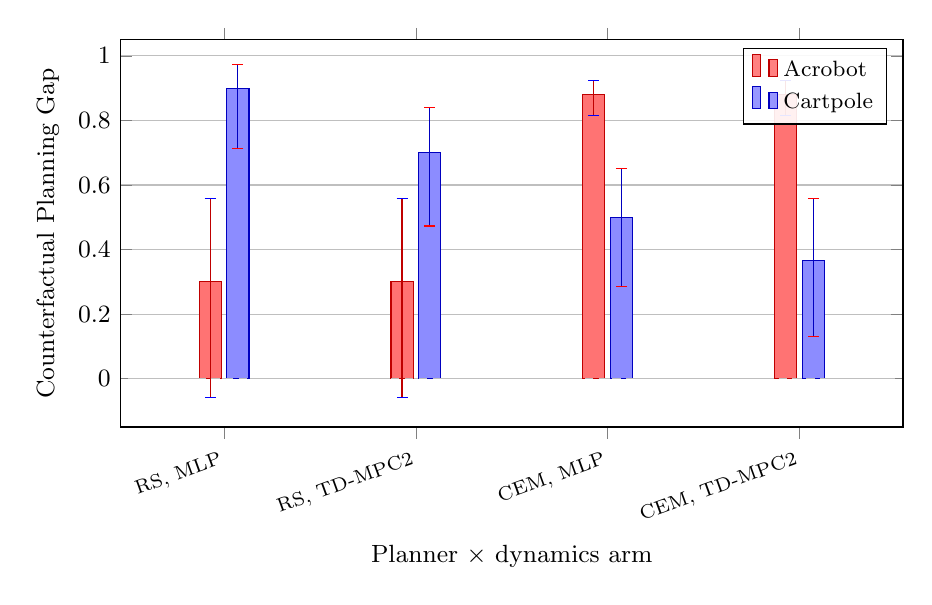
\begin{tikzpicture}
    \begin{axis}[
        width=0.95\columnwidth,
        height=6.5cm,
        font=\small,
        ybar=2pt,
        bar width=8pt,
        ymin=-0.15, ymax=1.05,
        ytick={0, 0.2, 0.4, 0.6, 0.8, 1.0},
        ylabel={Counterfactual Planning Gap},
        ymajorgrids=true,
        xtick={1, 2, 3, 4},
        xticklabels={
          {RS, MLP},
          {RS, TD-MPC2},
          {CEM, MLP},
          {CEM, TD-MPC2},
        },
        x tick label style={font=\scriptsize, rotate=20, anchor=north east},
        xlabel={Planner $\times$ dynamics arm},
        legend cell align=left,
        legend style={
          at={(0.98, 0.98)}, anchor=north east,
          font=\footnotesize,
          fill=white, fill opacity=0.9, draw opacity=1, text opacity=1,
        },
        enlarge x limits=0.18,
      ]
      \addplot+[
          fill=red!55, draw=red!75!black,
          error bars/.cd, y dir=both, y explicit,
        ]
        table[x=x, y=y, y error plus=eplus, y error minus=eminus, row sep=\\] {
          x y     eplus eminus \\
          1 0.300 0.259 0.359  \\
          2 0.300 0.259 0.359  \\
          3 0.880 0.043 0.066  \\
          4 0.880 0.043 0.066  \\
        };
      \addlegendentry{Acrobot}
      \addplot+[
          fill=blue!45, draw=blue!75!black,
          error bars/.cd, y dir=both, y explicit,
        ]
        table[x=x, y=y, y error plus=eplus, y error minus=eminus, row sep=\\] {
          x y     eplus eminus \\
          1 0.900 0.073 0.186  \\
          2 0.700 0.140 0.227  \\
          3 0.500 0.152 0.215  \\
          4 0.367 0.191 0.237  \\
        };
      \addlegendentry{Cartpole}
      \draw[densely dashed, gray!50] (axis cs:0.5, 0) -- (axis cs:4.5, 0);
    \end{axis}
  \end{tikzpicture}
  \caption{Cross-environment CPG with Agresti--Caffo $95\%$ CI error bars. Same four planner-dynamics combinations on two envs. Sample sizes: Acrobot random-shooting cells at $n = 10$, Acrobot CEM cells pooled at $n = 150$, Cartpole all four cells pooled at $n = 30$ (TD-MPC2 \texttt{model\_size}~$= 5$). The \textsc{model bottleneck} verdict reproduces in every cell; the gap magnitude differs and ranks the four arm configurations consistently within each env. The TD-MPC2 arm on Cartpole reaches non-zero learned-arm success ($0.200$ random-shooting, $0.133$ CEM), so the gap shrinks but stays bounded above zero -- the metric tracks gap magnitude, not just gap presence.}
  \label{fig:cross_env_cpg}
\end{figure}


% Figure: Cartpole capacity sweep. Same four arm configs as Figure 3,
% but comparing TD-MPC2 model_size=5 against model_size=1 within Cartpole.
%
% Data sources (all n=30 pooled across seeds {0,1,2}, 1M env steps):
%   model_size=5:
%     RS x MLP-on-TDMPC2-data : results/dmc_cartpole/coverage_mlp_on_tdmpc2_cpg_size5_pooled.json
%       gap=+0.900  CI=[+0.714, +0.973]   eplus=0.073  eminus=0.186
%     RS x TD-MPC2            : results/dmc_cartpole/tdmpc2_cpg_size5_pooled.json
%       gap=+0.700  CI=[+0.473, +0.840]   eplus=0.140  eminus=0.227
%     CEM x MLP-on-TDMPC2-data: results/dmc_cartpole/cem_cpg_size5_pooled.json
%       gap=+0.500  CI=[+0.285, +0.652]   eplus=0.152  eminus=0.215
%     CEM x TD-MPC2           : same file
%       gap=+0.367  CI=[+0.130, +0.558]   eplus=0.191  eminus=0.237
%   model_size=1:
%     RS x MLP-on-TDMPC2-data : results/dmc_cartpole/coverage_mlp_on_tdmpc2_cpg_pooled.json
%       gap=+0.900  CI=[+0.714, +0.973]   eplus=0.073  eminus=0.186
%     RS x TD-MPC2            : results/dmc_cartpole/tdmpc2_cpg_pooled.json
%       gap=+0.400  CI=[+0.167, +0.583]   eplus=0.183  eminus=0.233
%     CEM x MLP-on-TDMPC2-data: results/dmc_cartpole/cem_cpg_pooled.json cpgs.mlp_on_data
%       gap=+0.433  CI=[+0.206, +0.607]   eplus=0.174  eminus=0.227
%     CEM x TD-MPC2           : same file cpgs.tdmpc2
%       gap=-0.033  CI=[-0.276, +0.214]   eplus=0.247  eminus=0.243
\begin{figure}[t]
  \centering
  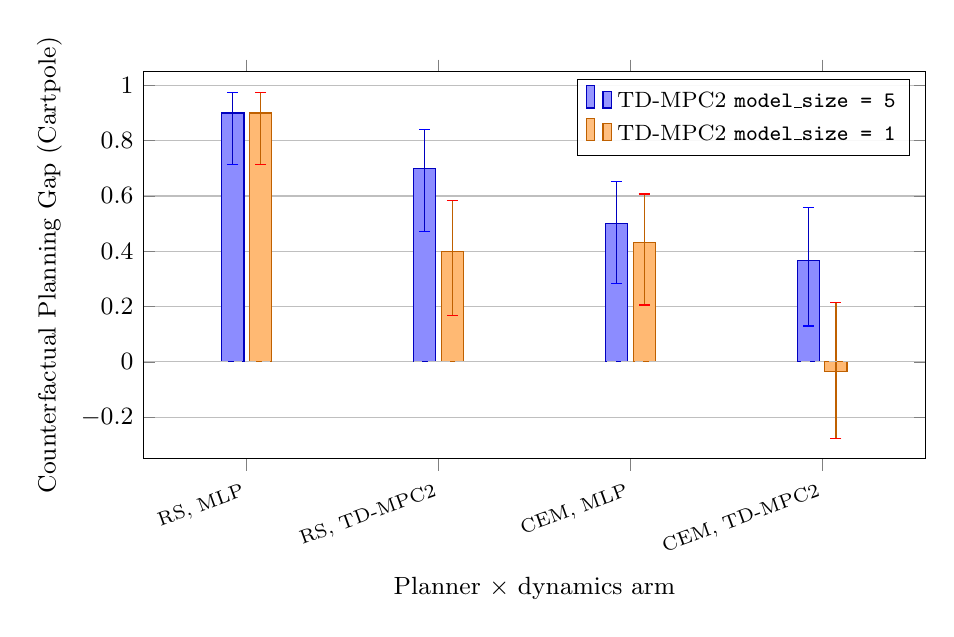
\begin{tikzpicture}
    \begin{axis}[
        width=0.95\columnwidth,
        height=6.5cm,
        font=\small,
        ybar=2pt,
        bar width=8pt,
        ymin=-0.35, ymax=1.05,
        ytick={-0.2, 0, 0.2, 0.4, 0.6, 0.8, 1.0},
        ylabel={Counterfactual Planning Gap (Cartpole)},
        ymajorgrids=true,
        xtick={1, 2, 3, 4},
        xticklabels={
          {RS, MLP},
          {RS, TD-MPC2},
          {CEM, MLP},
          {CEM, TD-MPC2},
        },
        x tick label style={font=\scriptsize, rotate=20, anchor=north east},
        xlabel={Planner $\times$ dynamics arm},
        legend cell align=left,
        legend style={
          at={(0.98, 0.98)}, anchor=north east,
          font=\footnotesize,
          fill=white, fill opacity=0.9, draw opacity=1, text opacity=1,
        },
        enlarge x limits=0.18,
      ]
      \addplot+[
          fill=blue!45, draw=blue!75!black,
          error bars/.cd, y dir=both, y explicit,
        ]
        table[x=x, y=y, y error plus=eplus, y error minus=eminus, row sep=\\] {
          x y     eplus eminus \\
          1 0.900 0.073 0.186  \\
          2 0.700 0.140 0.227  \\
          3 0.500 0.152 0.215  \\
          4 0.367 0.191 0.237  \\
        };
      \addlegendentry{TD-MPC2 \texttt{model\_size = 5}}
      \addplot+[
          fill=orange!55, draw=orange!75!black,
          error bars/.cd, y dir=both, y explicit,
        ]
        table[x=x, y=y, y error plus=eplus, y error minus=eminus, row sep=\\] {
          x y      eplus eminus \\
          1  0.900 0.073 0.186  \\
          2  0.400 0.183 0.233  \\
          3  0.433 0.174 0.227  \\
          4 -0.033 0.247 0.243  \\
        };
      \addlegendentry{TD-MPC2 \texttt{model\_size = 1}}
      \draw[densely dashed, gray!50] (axis cs:0.5, 0) -- (axis cs:4.5, 0);
    \end{axis}
  \end{tikzpicture}
  \caption{Cartpole capacity sweep at fixed $1 \times 10^{6}$-step training budget. Same four planner-dynamics combinations as Figure~\ref{fig:cross_env_cpg}, comparing TD-MPC2 \texttt{model\_size = 5} (blue) against \texttt{model\_size = 1} (orange), $n = 30$ pooled per bar with asymmetric AC error bars. The CEM~$\times$~TD-MPC2 cell at \texttt{model\_size = 1} (rightmost orange bar) is the only cell where the CI crosses zero: raw CPG $= -0.033$, AC CI $= [-0.28, +0.21]$, verdict \textsc{inconclusive}. Smaller-capacity TD-MPC2 closes the gap on Cartpole's CEM oracle that the larger-capacity model does not -- the metric reports this honestly rather than committing to a verdict the data does not support.}
  \label{fig:cartpole_capacity}
\end{figure}


Figure~\ref{fig:cross_env_cpg} aggregates the three environments on the same four arm configurations; Figure~\ref{fig:cartpole_capacity} shows the within-Cartpole capacity sweep that exposes the \textsc{inconclusive} cell.

\subsection{Power analysis: how many episodes before a ranking is trustworthy}
\label{sec:power}

The verdict gate turns from a post-hoc label into a planning tool once it is read forward: given hypothesised success rates and a target precision, how many episodes per arm does the AC interval need? Because the half-width depends only on the rates and $n$ (\S\ref{sec:cpg}), this is pure arithmetic, computable before any rollout. Table~\ref{tab:power} reports the per-arm $n$ needed to reach a half-width of $0.05$ (an interval of $\pm 5$ percentage points) for a range of oracle rates with the learned arm at $0$, the regime the worked examples occupy.

\begin{table}[t]
  \centering
  \small
  \begin{tabular}{rrrr}
    \toprule
    Oracle rate & $n$ for $\mathrm{hw}\!\le\!0.10$ & $n$ for $\mathrm{hw}\!\le\!0.05$ & $n$ for $\mathrm{hw}\!\le\!0.02$ \\
    \midrule
    $0.30$ & $84$  & $327$ & $2021$ \\
    $0.50$ & $98$  & $387$ & $2403$ \\
    $0.70$ & $84$  & $327$ & $2021$ \\
    $0.90$ & $46$  & $153$ & $881$  \\
    \bottomrule
  \end{tabular}
  \caption{Per-arm episode count needed to reach a target Agresti--Caffo half-width (learned arm at $0$, $z = 1.96$). Reproduced by \texttt{python -m experiments.power\_analysis}; numbers from \texttt{results/power\_analysis.json}.}
  \label{tab:power}
\end{table}

The same arithmetic audits a point-estimate leaderboard. Consider two systems reported at success rates $0.94$ and $0.92$ over $n = 100$ episodes per arm with no interval -- a plausible top-of-table near-tie. The AC interval on that difference has half-width $0.074$ and \emph{straddles zero}: the reported ranking gap is statistically indistinguishable from noise at the sample size used, and separating the two to a half-width of $0.05$ would require $n = 209$ per arm. A wider gap ($0.94$ vs $0.78$) is decidable at the same $n = 100$ ($\mathrm{hw} = 0.095$, interval clears zero); a mid-table near-tie ($0.78$ vs $0.75$) is not. This is the knowledge a leaderboard cannot carry: not which number is larger, but whether the ordering survives its own sample size. A reader holding only point estimates cannot tell a real ranking from a coin flip; the power table makes the distinction mechanical.

A traced decision closes the loop. The Cartpole \texttt{model\_size = 1}, CEM, TD-MPC2 cell returned \textsc{inconclusive} at $n = 30$ (half-width $0.245$). The table prescribes the per-arm count that would shrink the interval to a target precision and let the gate commit; reporting that number, rather than silently presenting an under-powered verdict as if it were decisive, is what \emph{decision-grade} is meant to denote.

% Figure: CPG verdict detectability map. For a top-of-leaderboard oracle
% rate (0.94), the boundary is the smallest oracle-minus-learned success-rate
% gap whose Agresti-Caffo CI clears zero at a given per-arm n -- i.e. the gap
% the five-branch verdict can actually commit on. Below the curve the gate
% returns INCONCLUSIVE; above it the ranking is decidable.
%
% Boundary computed by wmel.metrics.detectable_gap_at_n(0.94, 0.94 - g, n);
% values baked here so the figure is self-checking:
%   n:   10    20    30    50    75   100   150   200   300   500   1000
%   g: 0.415 0.260 0.195 0.140 0.110 0.090 0.070 0.060 0.045 0.035 0.025
%
% Annotated points (both at n=100): a leaderboard near-tie (gap 0.02) sits in
% the INCONCLUSIVE region; a wider gap (0.16) is decidable. Matches the
% leaderboard-gap audit in results/power_analysis.json.
\begin{figure}[t]
  \centering
  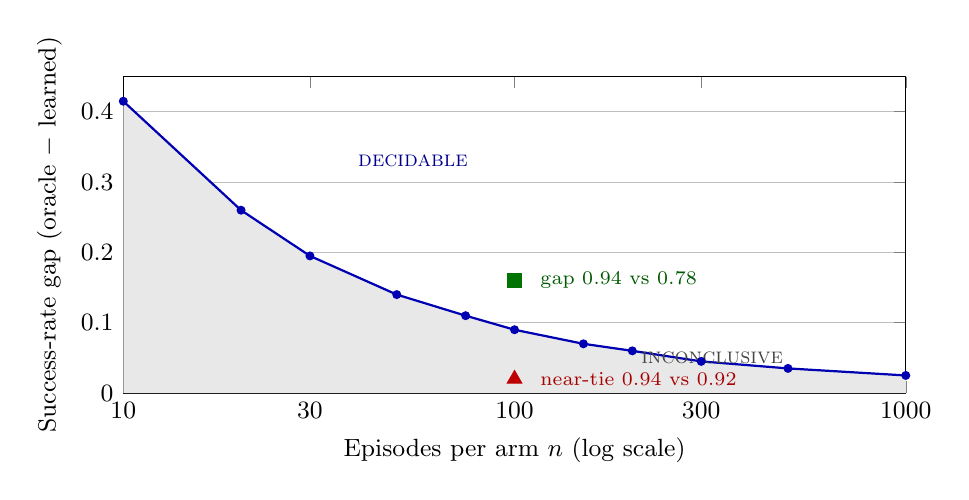
\begin{tikzpicture}
    \begin{axis}[
        width=0.95\columnwidth,
        height=5.6cm,
        font=\small,
        xmode=log, log basis x=10,
        xmin=10, xmax=1000,
        xtick={10, 30, 100, 300, 1000},
        xticklabels={$10$, $30$, $100$, $300$, $1000$},
        xlabel={Episodes per arm $n$ (log scale)},
        ymin=0, ymax=0.45,
        ytick={0, 0.1, 0.2, 0.3, 0.4},
        ylabel={Success-rate gap (oracle $-$ learned)},
        ymajorgrids=true,
        clip=false,
      ]
      % INCONCLUSIVE region: below the boundary (shade to the x-axis).
      \addplot[draw=none, fill=gray!18] coordinates {
        (10, 0.415) (20, 0.260) (30, 0.195) (50, 0.140) (75, 0.110)
        (100, 0.090) (150, 0.070) (200, 0.060) (300, 0.045) (500, 0.035) (1000, 0.025)
      } \closedcycle;
      % The decidability boundary itself.
      \addplot[color=blue!70!black, thick, mark=*, mark size=1.2pt] coordinates {
        (10, 0.415) (20, 0.260) (30, 0.195) (50, 0.140) (75, 0.110)
        (100, 0.090) (150, 0.070) (200, 0.060) (300, 0.045) (500, 0.035) (1000, 0.025)
      };
      % Region labels.
      \node[font=\footnotesize, gray!55!black] at (axis cs:320, 0.05) {\textsc{inconclusive}};
      \node[font=\footnotesize, blue!55!black] at (axis cs:55, 0.33) {\textsc{decidable}};
      % Annotated leaderboard points at n=100.
      \addplot[only marks, mark=triangle*, mark size=3pt, color=red!75!black]
        coordinates {(100, 0.02)};
      \node[font=\scriptsize, red!65!black, anchor=west] at (axis cs:110, 0.02)
        {near-tie $0.94$ vs $0.92$};
      \addplot[only marks, mark=square*, mark size=2.6pt, color=green!45!black]
        coordinates {(100, 0.16)};
      \node[font=\scriptsize, green!35!black, anchor=west] at (axis cs:110, 0.16)
        {gap $0.94$ vs $0.78$};
    \end{axis}
  \end{tikzpicture}
  \caption{Verdict detectability map at oracle rate $0.94$. The curve is the smallest oracle-minus-learned success-rate gap whose Agresti--Caffo $95\%$ CI clears zero at a given per-arm $n$ (computed by \texttt{detectable\_gap\_at\_n}). Below it the gate returns \textsc{inconclusive}; above it the ranking is decidable. A leaderboard near-tie ($0.94$ vs $0.92$, gap $0.02$) reported at $n = 100$ (red triangle) sits inside the \textsc{inconclusive} region -- the ordering is not supported by its own sample size; a wider gap ($0.94$ vs $0.78$, green square) is decidable at the same $n$. A point estimate cannot show which side of this boundary a reported ranking sits on.}
  \label{fig:power_detectability}
\end{figure}


Figure~\ref{fig:power_detectability} draws the same fact as a decision boundary: at a fixed oracle rate, the smallest success-rate gap the verdict can commit on shrinks with $n$, and a reported ranking sits on one side of that boundary or the other. The near-tie at $n = 100$ falls inside the \textsc{inconclusive} region; only a wider gap, or a larger $n$, crosses into the decidable region.

\section{Discussion and Limitations}

The empirical study spans three DMC control tasks (Acrobot-swingup, Cartpole-swingup, Reacher-easy), two planners (random-shooting and CEM), two learned-dynamics families (a bespoke MLP and TD-MPC2), and multi-seed pooling up to $n = 150$ per arm. It remains deliberately scoped to simulated, fully-observed control where an oracle dynamics is available: the methodological contribution -- a packaged CPG with an Agresti--Caffo CI, a gated verdict, and a power table -- is decoupled from any of those choices but does require an oracle. On hardware-in-the-loop or physical environments the metric is undefined; surrogate CPG variants (e.g.\ a higher-fidelity model standing in for the oracle, or a domain-randomised reference in the spirit of \citet{tobin2017domain}) are future work.

The framework's adapter interface (\S\ref{sec:framework}) is what makes CPG cheap to compute: any \texttt{dynamics} callable can be swapped into the same planner without touching anything else, any planner can be swapped against a fixed dynamics, and any perturbation can be plugged into the runner. \S\ref{sec:robustness} through \S\ref{sec:reacher} exercised this on a published world model (TD-MPC2), on a CEM planner, on a pooled-$150$ multi-seed extension under CEM, on an action-burst perturbation sweep, and on two further environments (Cartpole-swingup and Reacher-easy); the verdict is robust across all of them, the random-shooting MPC was bracketing the Acrobot oracle low, and the pooled CI half-widths are below $0.06$ where pooled to $n=150$. Natural further axes that the same plumbing supports are a continuous-return variant of CPG (the difference of mean returns rather than success rates), a pooled-$150$ tightening of the Cartpole and Reacher cells (presently $n=30$), and a learned score function that removes the task-specific scoring heuristic.

\paragraph{Properties and threats to validity.} Three properties bound what CPG can claim, and we state them explicitly rather than leave them for a reader to infer. First, \textbf{CPG's magnitude is a function of the oracle planner's strength, not only the model.} The gap moves from $+0.30$ under random-shooting MPC to $+0.88$ under CEM (\S\ref{sec:robustness}) with the learned arm pinned at $0$ throughout: a stronger oracle planner inflates the gap without any change to the model. The point estimate should therefore be read relative to a stated planner, and CPG is best used to \emph{rank} dynamics callables under a fixed planner or to power a verdict, not as a planner-free absolute. The verdict gate inherits this only weakly, because it asks whether the interval clears zero, not where the point estimate sits. Second, \textbf{the load-bearing demonstration of the metric is the cell where the verdict changes its decision}, not the cells where the learned arm is at $0/n$. Where an arm is pinned at zero, any sane estimator agrees the oracle is better and the metric is merely confirming the obvious; the genuinely informative behaviour is the Cartpole \texttt{model\_size}~$=1$, CEM, TD-MPC2 cell (\S\ref{sec:crossenv}), where the learned arm reaches $0.533$ against an oracle at $0.500$ and the gate returns \textsc{inconclusive} rather than convicting either side. A gate that flips on the strength of the evidence is the property a point-estimate leaderboard cannot reproduce. Third, \textbf{the metric requires an oracle dynamics callable and is therefore confined to simulated environments} where state can be reconstructed and re-stepped; our own Acrobot oracle reconstructs $(q_{\mathrm{pos}}, q_{\mathrm{vel}})$ lossily modulo $2\pi$ and re-steps MuJoCo. This is a hard scope wall, not a tuning detail: CPG does not extend to the sim-to-real regime without a surrogate-oracle variant, which we leave to future work.

Other limitations worth flagging explicitly. The discrete-torque action space is a five-level approximation of the continuous control problem; a continuous variant of CEM over a Gaussian per-timestep mean is a straightforward extension. The Acrobot success criterion ($r_t \geq 0.6$) is a binary projection of a dense reward; a continuous variant of CPG that reports the difference of mean returns is straightforward and may be more sample-efficient. The planner score is task-specific and tightly coupled to the environment's reward geometry; a learned score function (predicting the DMC reward directly from the latent state) would remove this coupling, at the cost of a second model component.

\section{Conclusion}

We have proposed the Counterfactual Planning Gap as a decision-grade metric for world-model evaluation, packaged it behind a minimal evaluation contract, and reported a worked example on DMC Acrobot-swingup. At $n = 10$ under random-shooting MPC the framework reports \textsc{inconclusive}; pooled-$150$ tightens the CI off zero and returns \textsc{model bottleneck}; sweeping the training-set size across nearly three orders of magnitude leaves the verdict unchanged while the held-out prediction loss drops by $\sim 150\times$. The robustness sweep in \S\ref{sec:robustness} adds a published-world-model arm (TD-MPC2) and a CEM planner: both learned arms remain at $0$ success, the oracle's success rate triples under CEM ($0.30 \to 0.90$), and the gap opens to $+0.900$ with a CI that no longer crosses zero at $n = 10$. A pooled-$150$ extension of the CEM rows tightens this to $+0.880$, CI $[+0.814, +0.923]$, with both learned arms still at $0/150$. An action-burst perturbation sweep (\S\ref{sec:robustness_perturbation}) confirms the verdict survives a per-episode \texttt{DropNextActions}$(k)$ at $k \in \{0, 1, 5\}$. A cross-environment replay on DMC Cartpole-swingup (\S\ref{sec:crossenv}) reproduces \textsc{model bottleneck} in every cell at TD-MPC2 \texttt{model\_size} $= 5$, produces the paper's first non-trivial learned-arm successes (TD-MPC2 dynamics reaches $0.200$ and $0.133$ under random-shooting and CEM respectively, both still \textsc{model bottleneck} because the gap is bounded above zero), and -- at the smaller \texttt{model\_size} $= 1$ checkpoint -- delivers the paper's first moderate-$n$ \textsc{inconclusive} verdict on the CEM~$\times$~TD-MPC2 cell, where the smaller-capacity model matches the oracle ($0.533$ vs $0.500$) and the CI crosses zero. A third environment, Reacher-easy (\S\ref{sec:reacher}), gives the cleanest case: the oracle reaches the target in every cell ($1.000$) and both learned arms are clearly non-zero ($0.300$--$0.633$), so all four cells are \textsc{model bottleneck} on genuine, non-degenerate gaps and the verdict ranks the two learned dynamics by how much planning success each forfeits. The takeaway is methodological: a metric that separates closed-loop success from prediction quality reveals two distinct contributors that prediction-quality metrics alone would conflate -- a coverage-or-capacity dynamics-quality bottleneck on the learned arms, and a planner-capacity contributor on the oracle arm -- and an adapter-and-planner interface that lets a single \texttt{BenchmarkRunner} disentangle them by swapping callables; the verdict travels across the easy/hard env axis at fixed family and tracks gap magnitude rather than only gap presence. We argue this kind of calibrated honesty -- a metric that refuses to claim more than the data supports, and that supports a precise attribution once the data is sufficient -- is the right design target for a methodology paper that wants to sit usefully next to a fast-moving model literature.

\section*{Acknowledgements}

This work is independent. It is not affiliated with the AMI (Advanced Machine Intelligence) program at Meta, the LeWorldModel project, the authors of any of the cited papers, or any current or past employer of the author. The repository was developed end-to-end with an LLM coding agent in the loop (Claude Code); a description of the development recipe and the pre-tag adversarial-review pattern that caught most of the metric-correctness bugs along the way is included in the repository at \texttt{docs/process/llm\_agent\_recipe.md}.

\bibliographystyle{plainnat}
\bibliography{references}

\end{document}
